%%%%%%%%%%%%%%%%%%%%%%%%%%%%%%%%%%%%%%%%%
% Structured General Purpose Assignment
% LaTeX Template
%
% This template has been downloaded from:
% http://www.latextemplates.com
%
% Original author:
% Ted Pavlic (http://www.tedpavlic.com)
%
% Note:
% The \lipsum[#] commands throughout this template generate dummy text
% to fill the template out. These commands should all be removed when 
% writing assignment content.
%
%%%%%%%%%%%%%%%%%%%%%%%%%%%%%%%%%%%%%%%%%

\documentclass{article}

\usepackage{fancyhdr} % Required for custom headers
\usepackage{lastpage} % Required to determine the last page for the footer
\usepackage{extramarks} % Required for headers and footers
\usepackage{graphicx} % Required to insert images
\usepackage[utf8]{inputenc}

% Margins
\topmargin=-0.45in
\evensidemargin=0in
\oddsidemargin=0in
\textwidth=6.5in
\textheight=9.0in
\headsep=0.25in 

\linespread{1.1} % Line spacing



\setlength\parindent{0pt} % Removes all indentation from paragraphs

%----------------------------------------------------------------------------------------
%	DOCUMENT STRUCTURE COMMANDS
%	Skip this unless you know what you're doing
%----------------------------------------------------------------------------------------

% Header and footer for when a page split occurs within a problem environment
\newcommand{\enterProblemHeader}[1]{
\nobreak\extramarks{#1}{#1 continued on next page\ldots}\nobreak
\nobreak\extramarks{#1 (continued)}{#1 continued on next page\ldots}\nobreak
}

% Header and footer for when a page split occurs between problem environments
\newcommand{\exitProblemHeader}[1]{
\nobreak\extramarks{#1 (continued)}{#1 continued on next page\ldots}\nobreak
\nobreak\extramarks{#1}{}\nobreak
}

\setcounter{secnumdepth}{0} % Removes default section numbers
\newcounter{homeworkProblemCounter} % Creates a counter to keep track of the number of problems

%----------------------------------------------------------------------------------------
%	NAME AND CLASS SECTION
%----------------------------------------------------------------------------------------

\newcommand{\lessonNumber}[1]{Lezione\ \##1} % Assignment title
\newcommand{\lessonDate}[4]{#1,\ #2\ #3\ #4} % Due date
\newcommand{\lessonCourse}[1]{#1} % Course/class
\newcommand{\lessonTime}[1]{#1} % Class/lecture time
\newcommand{\lessonTeacher}[1]{#1} % Teacher/lecturer
\newcommand{\lessonAuthor}[1]{#1} % Your name
\begin{document}

\section{Misurazione del codice(13)}

\textbf{Misurazione:} Processo che assegna numeri o simboli ad attributi di entità per descriverle secondo regole definite.
\textbf{Misura:} Assegnazione empirica e oggettiva di un valore ad un'entità per caratterizzarne un attributo specifico.
\textbf{Metrica:} insieme di regole per fissare entità da misurare gli attributi rilevanti, l'unità di misura. Secondo IEEE misura quantitativa del grado di possesso di uno specifico attributo da parte di un sistema, componente, processo.

Ci sono anche gli \textbf{indicatori} che sono delle misure indirette ottenute tramite stime o precisazioni. Gli obbiettivi nella misurazione SW sono quelli di valutare lo stato di:
\begin{itemize}
	\item Progetti, stime, preventivi e consuntivi di costo, tempo;
	\item Prodotti qualità;
	\item Processi qualità e miglioramenti;
	\item Risorse consumo;
\end{itemize}

\textbf{ISO 15939} the information needs are based on goals, constraints, risk, and problems which originate from the technical and mgmgt processes. Il CMMI suggerisce di determinarli nelle seguenti aree:
\begin{itemize}
	\item Requirements Management, quando le pratiche in uso aderiscono a quelle di riferimento e i prodotti del progetto soddisfano i requisiti;
	\item Design \& Implementation;
	\item Verification \& Validation;
	\item Quality Assurance, come \textit{requirements management};
	\item Configuration Management, quale è l'impatto di una data modifica e qual'è il grado di integrità delle baseline di progetto;
	\item Project Management, quanto sono affidabili i preventivi e accurati i consuntivi, quanto sono efficaci le misure correttive e quanto sono concretamente adottate;
	\item Risk analysis \& decision analysis, quali e quanto i rischi gravano attualmente sul progetto;
	\item Training.
\end{itemize}

\textbf{Metrica di project management:}

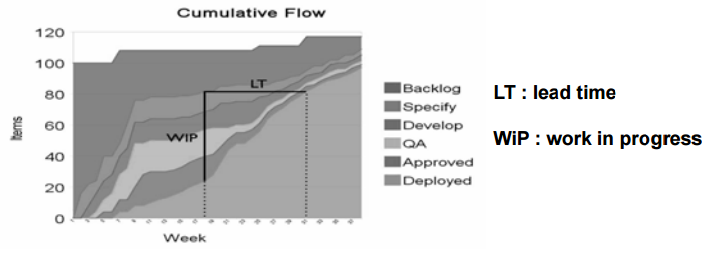
\includegraphics[width=0.5\columnwidth]{img1} % Example image

lead time= tempo che intercorre da quando un'azione è assegnata a quando ha avuto successo.

\textbf{Metriche software:}
\begin{itemize}
	\item \textbf{SLOC:} linee di codice sorgente, viene usata per derivare informazioni di costo e produttività, è solitamente rapportata con la densità di commenti. Tuttavia dipende dalla sintassi del linguaggio e dallo stile di codifica.
	\item \textbf{Complessità ciclomatica:} è  una metrica indipendente dal linguaggio, si svolge una misurazione astratta di un attributo significativo del software, misura la complessità del flusso di controllo e il grado di \textit{fan-in} \textit{fan-out} applicato hai dati può aiutare a stimare la complessità del flusso di dati, meglio comunque calcolarlo con strumenti automatici. L'unico difetto è che è molto onerosa da applicare prima della progettazione in dettaglio.\\
	\begin{center}
		v(G)=e-n+p
	\end{center}
	\begin{itemize}
		\item v(G), numero di percorsi lineari in G;
		\item e, numero degli archi (flusso);
		\item n, numero dei nodi (espressioni o comandi);
		\item p, numero delle componenti connesse ad ogni arco (p=2 per esecuzione sequenziale: 1 predecessore, 1 successore).
	\end{itemize}		
	
\end{itemize}

Le misure si dividono in due categorie, quelle interne (numero di requisiti, grado di coesione...) e quelle esterne (ISO/IEC 9126-1).\\
Per il software ad oggetti servono delle metriche:
\begin{itemize}
	\item Metodi, si può usare McCabe come metrica base (\textit{tiene conto di interfacce e variabili locali})\\
	\begin{center}
		MC=w1MIC+w2MLVC+w3MCC
	\end{center}
	\begin{itemize}
		\item MIC, complessità dell'interfaccia del metodo;
		\item MLVC, complessità delle variabili locali;
		\item MCC, complessità ciclomatica del codice;
		\item wi, preso determinato statisticamente.
	\end{itemize}
	\item Classe 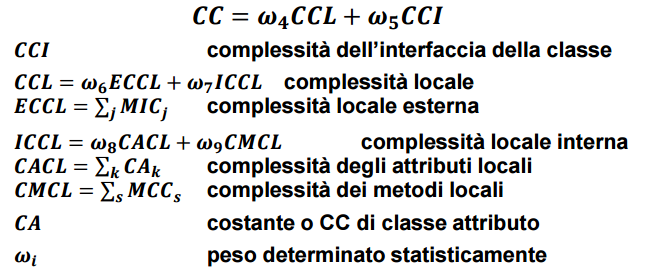
\includegraphics[width=0.5\columnwidth]{img2} % Example image
	\item Sistemi, 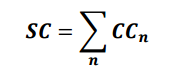
\includegraphics[width=0.1\columnwidth]{img3} % Example image
\end{itemize}

Bisogna in oltre prestare attenzione alla qualità delle metriche, qualità che si divide in precisione, aderenza alla realtà e accuratezza.
\end{document}